\section{Showcase for the Dark QCD model}
\label{darksec}

The arguments discussed before can be illustrated using a concrete physics scenario for BSM models.
In particular, we will consider the dark QCD model \cite{Bai:2013xga,Schwaller:2015gea}. It predicts 
the existence of the so-called ``emerging'' jets 
that are created in the decays of new long-lived neutral 
particles (dark hadrons), produced in a parton-shower process by dark QCD.
The process includes  two mediators with masses $Mx$, each of which 
decays promptly to a SM quark and a dark quark. 
The final-state signature consists of four jets with high transverse momenta, with two  
`emerging'' jets originating from ``dark'' quarks.  Such jets  contain many displaced
vertices arising from the decays of the dark pions produced in the dark parton shower.

Recently searches for the  emerging jets in $pp$ collisions have been performed \cite{Sirunyan:2018njd} 
by the CMS Collaboration.
The emerging jet contains multiple displaced vertices and multiple 
tracks with large impact parameters. Assuming that the mass of the dark pion is 5~GeV, 
the signal acceptance using this approach does not exceed 40\% at large masses of the mediators
(see Figure~4 of \cite{Sirunyan:2018njd}).
The decay length of a dark pion defines the distance from the interaction vertex of $pp$ collisions 
to the point where the jet emerges. The  emerging jet contains multiple displaced vertices
that are reconstructed using a tracker  \cite{Sirunyan:2018njd}.

Alternatively, emerging jets can be reconstructed using calorimeters with high-resolution time measurements. This method is expected
to have advantages for the measurements of dark pions with a large decay length, i.e. in the situations where the tracker has a low
reconstruction acceptance and resolution since only a few outer layers can be used for track reconstruction.
It was also pointed out \cite{Schwaller:2015gea} that the emerging jets may have significant fraction of neutral particles and the reconstruction
using charged tracks can have a low acceptance.

To estimate the performance of the timing layers in reconstructing emerging jets,
we will use the same Monte Carlo settings as for Ref.~\cite{Sirunyan:2018njd}:
The $pp$ collision event samples  were  generated with the ``hidden valley'' model framework in PYTHIA 8.2 assuming a centre-of-mass energy of 13~TeV and  
a fixed mass of 5~GeV for the dark pions. The samples were created after changing the decay distance $c\tau$ of the dark pions.  
The  mass $Mx$ of the mediator was also varied. 

To calculate the detector acceptance, the semi-analytical formalism based on Eq.~\ref{eqTOF} is used. In this relation $L=c\tau$ is the distance traveled
by the dark pion with a mass $m$ before it decays to the emerging jet.  
After the dark pion creates a SM jet, we assume that
such emerging jets travel to the surface of the timing layer with the speed of light for all values of $m$.
This is naturally to expect since the emerging SM jets consist of light stable particles (mostly photons and pions).
  
For the timing layers, the signature of emerging jets is time delays compared to the other SM jets. The  production vertex
cannot be observed by the timing layers if such jets emerge before TL1.
After events are generated, the weighted averages of the decay distances of all particles that originate from
the dark pions, using the particle momentum as the weight, were  calculated. This decay distance is used
to approximate the decay length, without using applying a jet reconstruction.  
The  calculation for the $3\sigma$ separation assumes $m_F=m_{\alpha}\simeq 3.73$~GeV although such a choice can be rather arbitrary.
This value of $m_F$ is used to give a conservative\footnote{One can argue that the SM jets mainly consist of light-flavour hadrons and photons, 
therefore, $m_F$ is significantly lower.} estimate of the arrival time of the emerging SM jets.

The acceptance of reconstruction of the emerging jet events was calculated by counting the number of events that pass the 
Eq.~\ref{eqTOF} condition  with the parameters as discussed before, divided by the total number of entries
without this requirement. Figure~\ref{fig:efficiency_med} shows the acceptance as a function of the mediator mass $Mx$ and the decay distance
of the dark pions. This figure can directly be compared to the similar acceptance figure for the method based on tracks  \cite{Sirunyan:2018njd}. 
The acceptance based on the TOF is significantly larger for low $Mx$ and large $L=c\tau$ of the dark pions, compared to a
similar acceptance distribution based on tracking information.  
The acceptance is larger for the timing layers with a resolution smaller than 100~ps, than for the standard 1-ns calorimeter resolution. 

Now we will be interested in the acceptance  of the reconstruction of dark pions  as a function of their mass
and their lifetime assuming a fixed mass $Mx$ of the mediator. This time we will consider the HE-LHC environment 
with $pp$ collisions at a centre-of-mass energy of 27~TeV.    
The Monte Carlo settings for the signal model were similar
to those discussed in  \cite{Sirunyan:2018njd,prive}.
The mass of the mediator was set to 10~TeV, while the mass of the dark pion was varied in the range between 5~GeV and 1~TeV.
The dark pion decay length, $c\tau$,  was varied between 1~mm and 1000~mm (independent of its mass). Other parameters
were also appropriately modified to allow a sufficient phase space for the dark meson production.
The mass of the dark pion is assumed to be one half the mass of the dark quark. The mass of the dark
$\rho$ is four times of the dark pion mass. The width of the
mediator particle is assumed to be small as compared to the detector mass resolution.

As before, the acceptance of reconstruction of the emerging jets by measuring the timing information was calculated by 
counting the number of events that pass the 
Eq.~\ref{eqTOF} condition  with the parameters as discussed before, divided by the total number of entries
without this requirement. Figure~\ref{fig:efficiency} shows the efficiency
as a function of $c\tau$ and the mass of the dark pion. It can be seen that a detector with the standard 1-ns resolution does
not have acceptance for the dark meson measurements. The acceptance is significantly larger for the timing layers that have a resolution smaller than 100~ns.
The acceptance is small for small $c\tau$ or small masses, which is the expected feature of the timing measurement.
The timing layers with 20-ps resolution have 100\% acceptance for large values of $c\tau$ and dark-meson masses.
The efficiency as a function of the particle velocity for the timing layers with the 20-ps and 1-ns resolutions
is shown in the \ref{appendix}.

Note that the obtained results are relatively general since they are formulated in the terms of masses and decay lengths,  
i.e. independent of the position of the timing layers and other details relevant to 
the detector geometry.


\begin{figure}
\begin{center}
   \subfigure[10 ps] {
   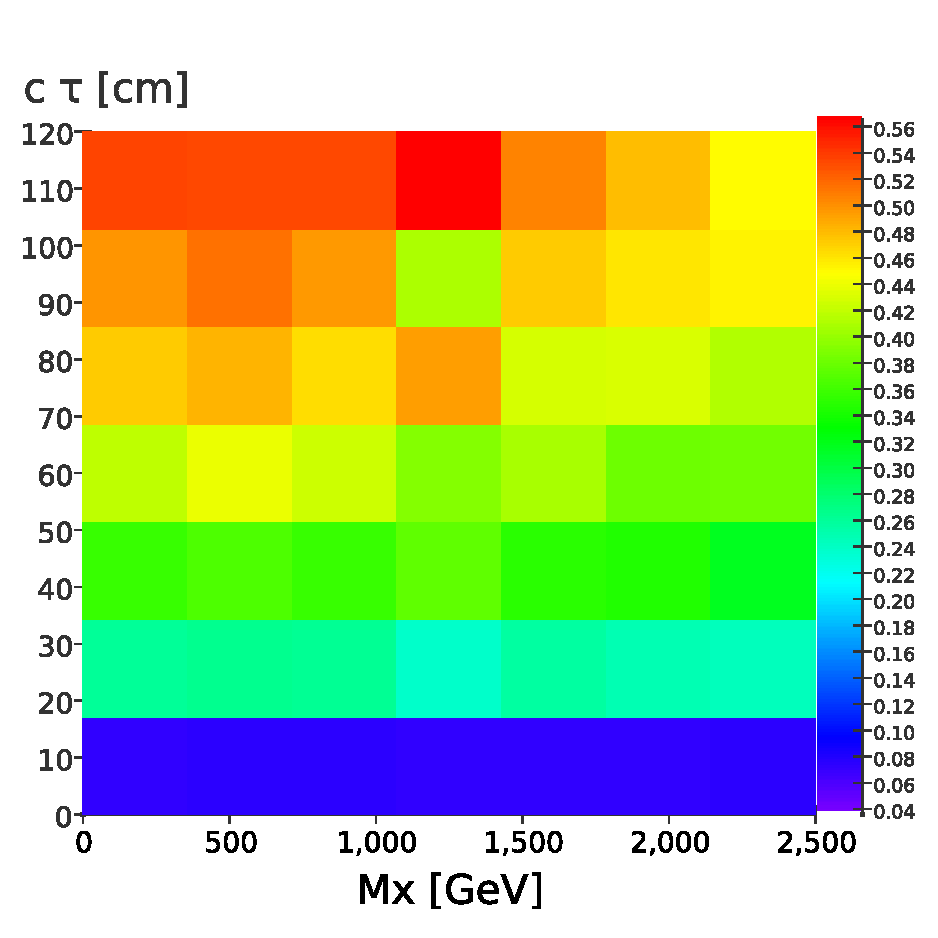
\includegraphics[width=0.4\textwidth]{effic10a_med.pdf}
   }
   \subfigure[20 ps] {
   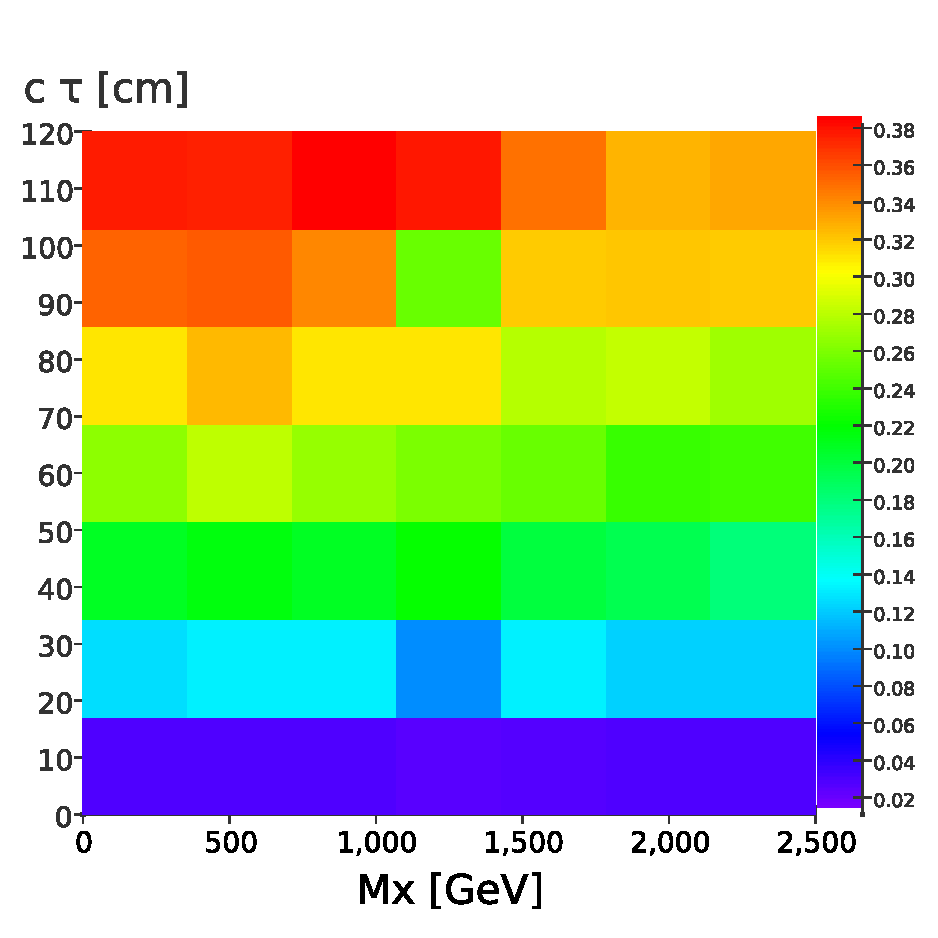
\includegraphics[width=0.4\textwidth]{effic20a_med.pdf}\hfill
   }

   \subfigure[30 ps] {
   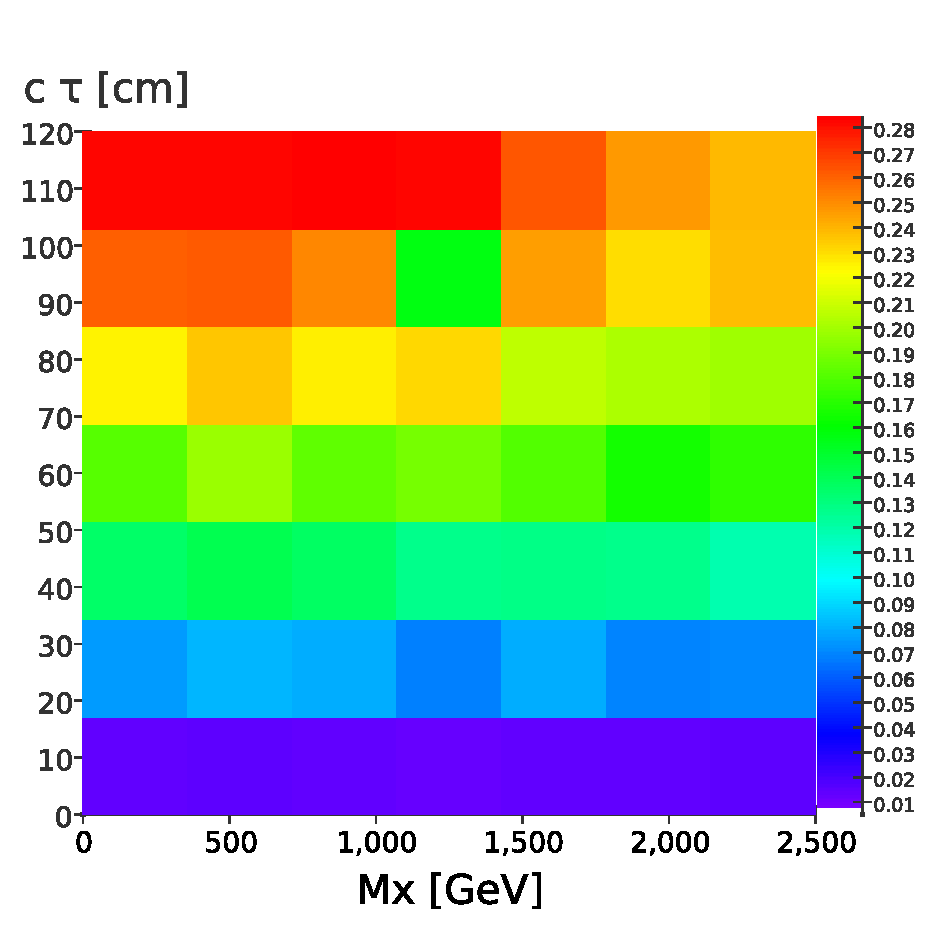
\includegraphics[width=0.4\textwidth]{effic30a_med.pdf}
   }
   \subfigure[100 ps] {
   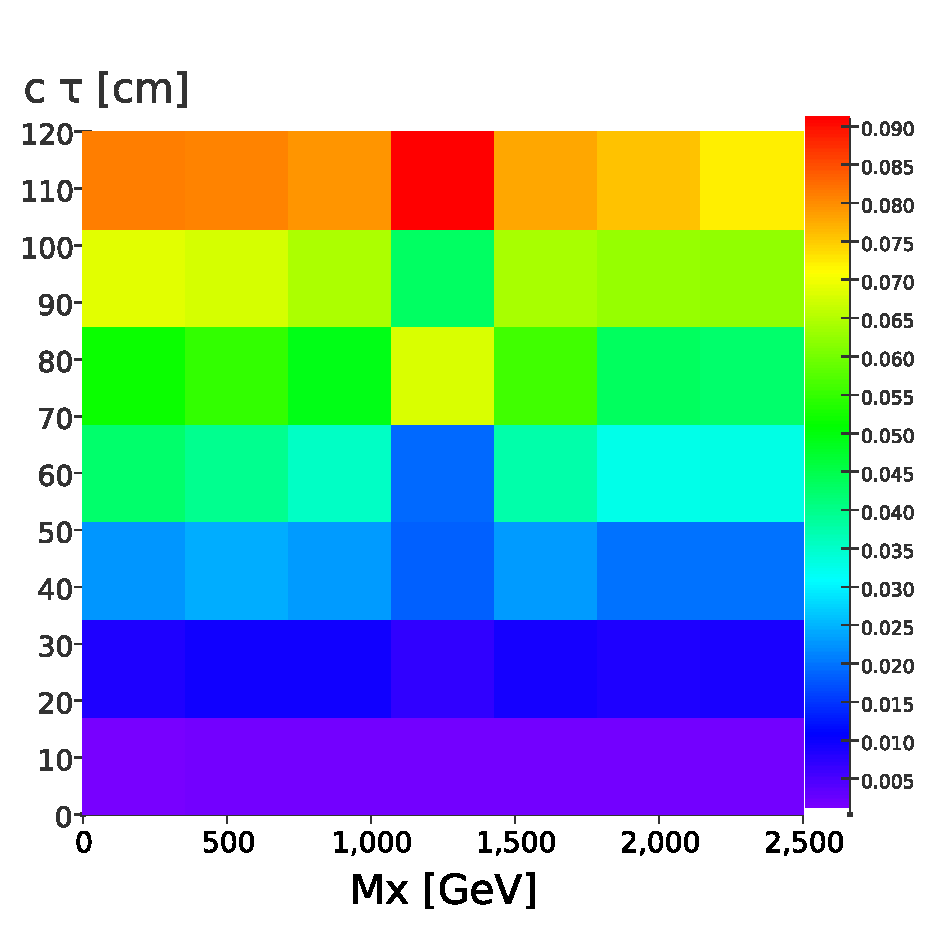
\includegraphics[width=0.4\textwidth]{effic100a_med.pdf}\hfill
   }

   \subfigure[500 ps] {
   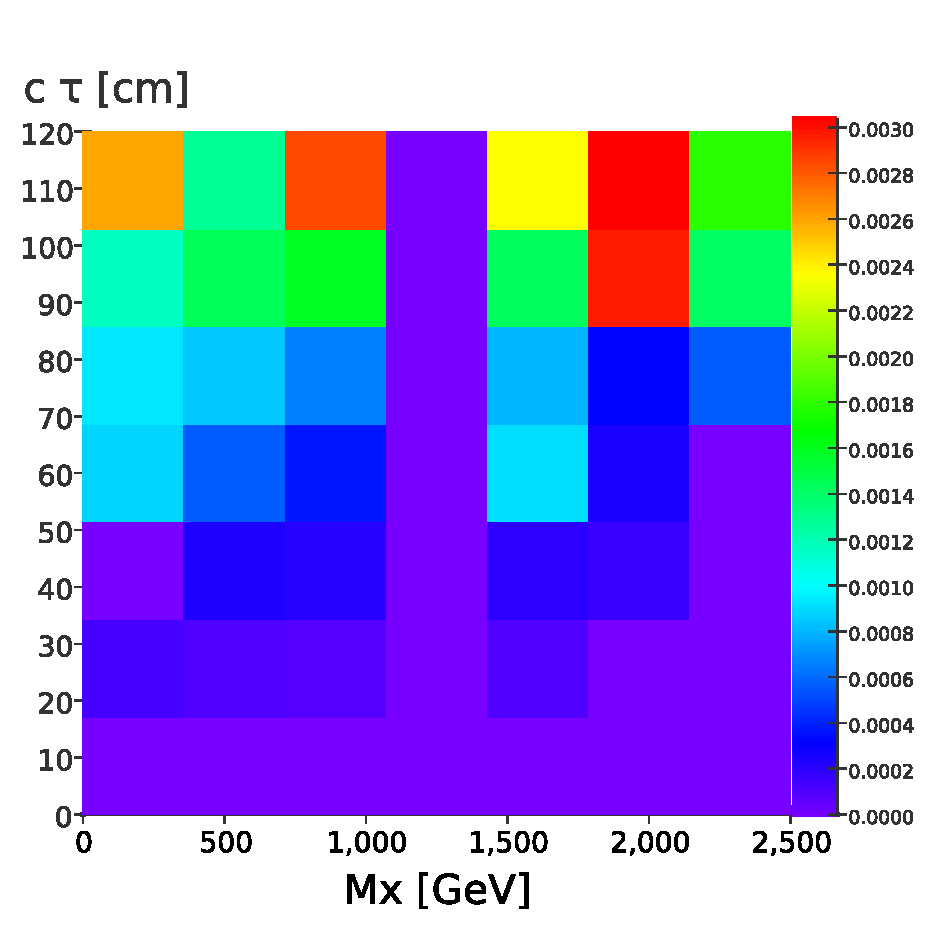
\includegraphics[width=0.4\textwidth]{effic500a_med.pdf}
   }
   \subfigure[1000 ps] {
   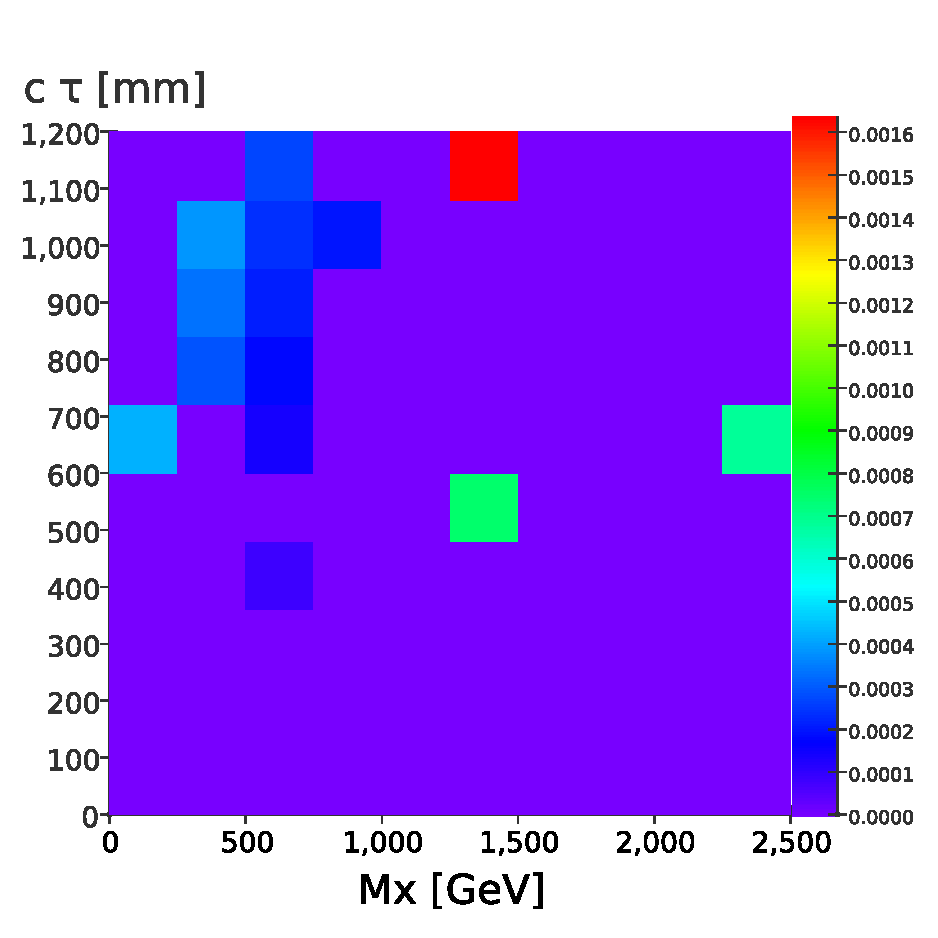
\includegraphics[width=0.4\textwidth]{effic1000a_med.pdf}\hfill
   }

\end{center}
\caption{
The acceptance for the reconstruction of emerging jets using the timing layers with different timing resolutions as
a function of the mediator mass $Mx$ and the $c\tau$ of the dark pions with the mass of 5~GeV.
The PYTHIA8 simulations are performed
for the $pp$ collisions at $\sqrt{s}=13$~TeV. 
}
\label{fig:efficiency_med}
\end{figure}



\begin{figure}
\begin{center}
   \subfigure[10 ps] {
   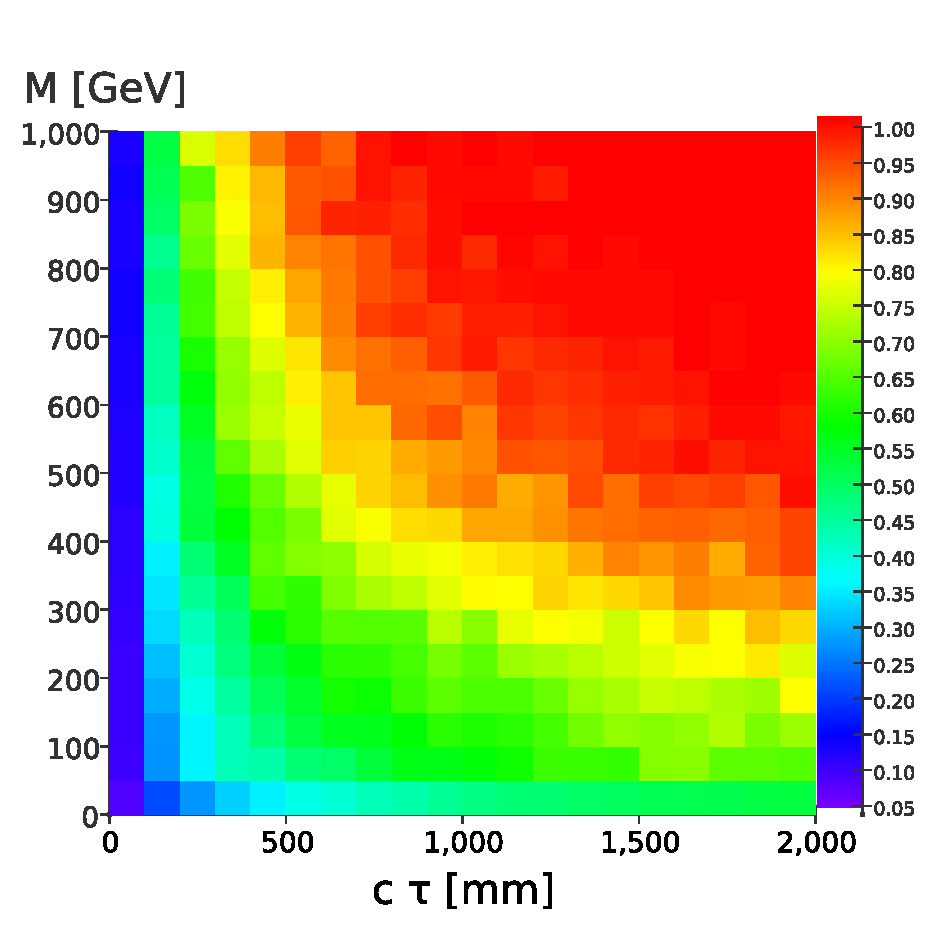
\includegraphics[width=0.4\textwidth]{effic10a.pdf}
   }
   \subfigure[20 ps] {
   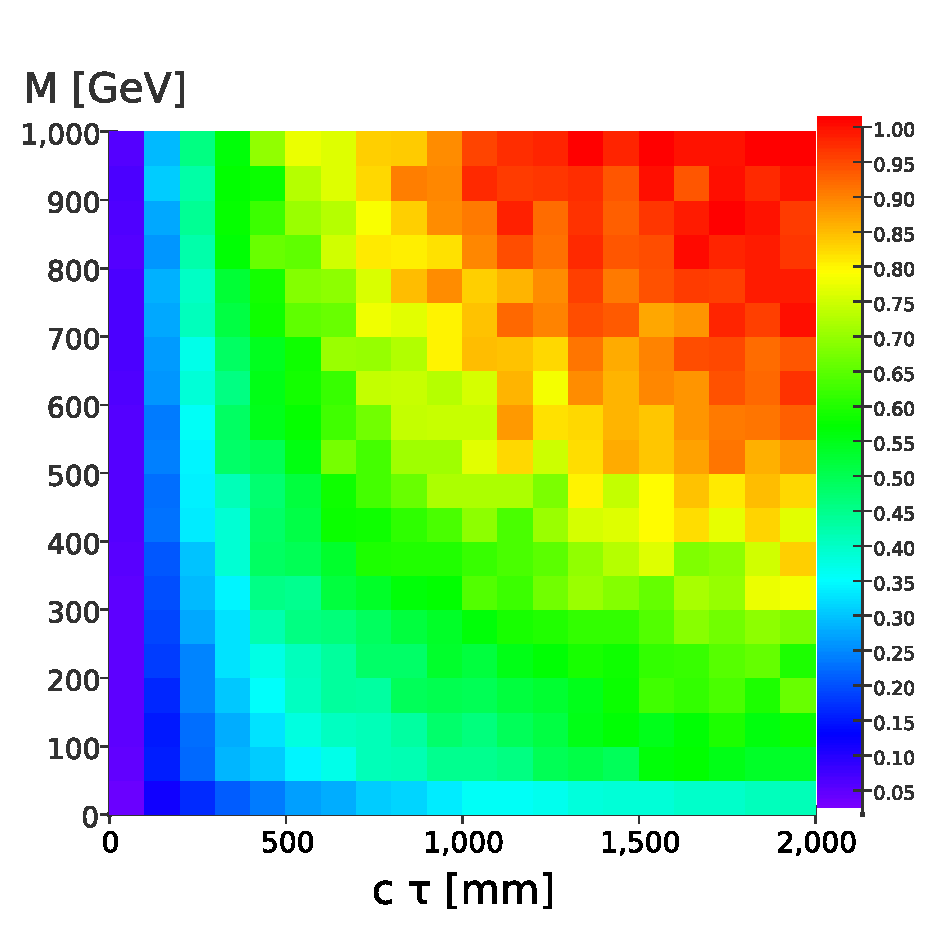
\includegraphics[width=0.4\textwidth]{effic20a.pdf}\hfill
   }

   \subfigure[30 ps] {
   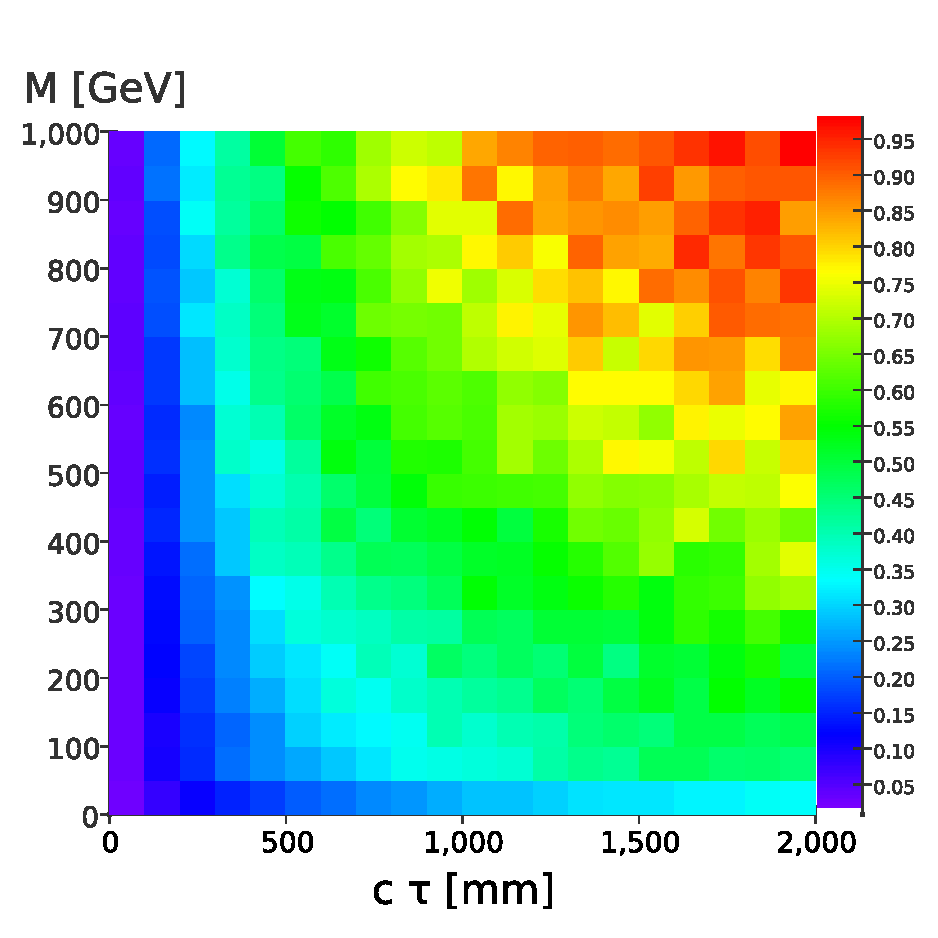
\includegraphics[width=0.4\textwidth]{effic30a.pdf}
   }
   \subfigure[100 ps] {
   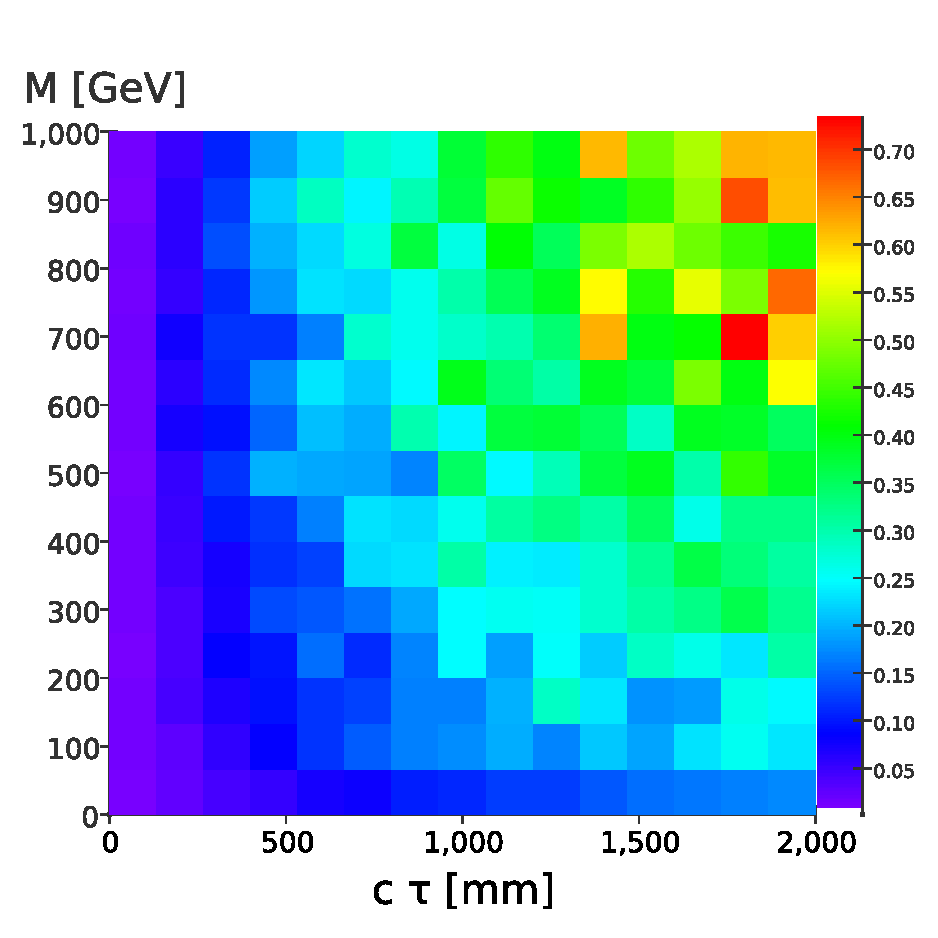
\includegraphics[width=0.4\textwidth]{effic100a.pdf}\hfill
   }

   \subfigure[500 ps] {
   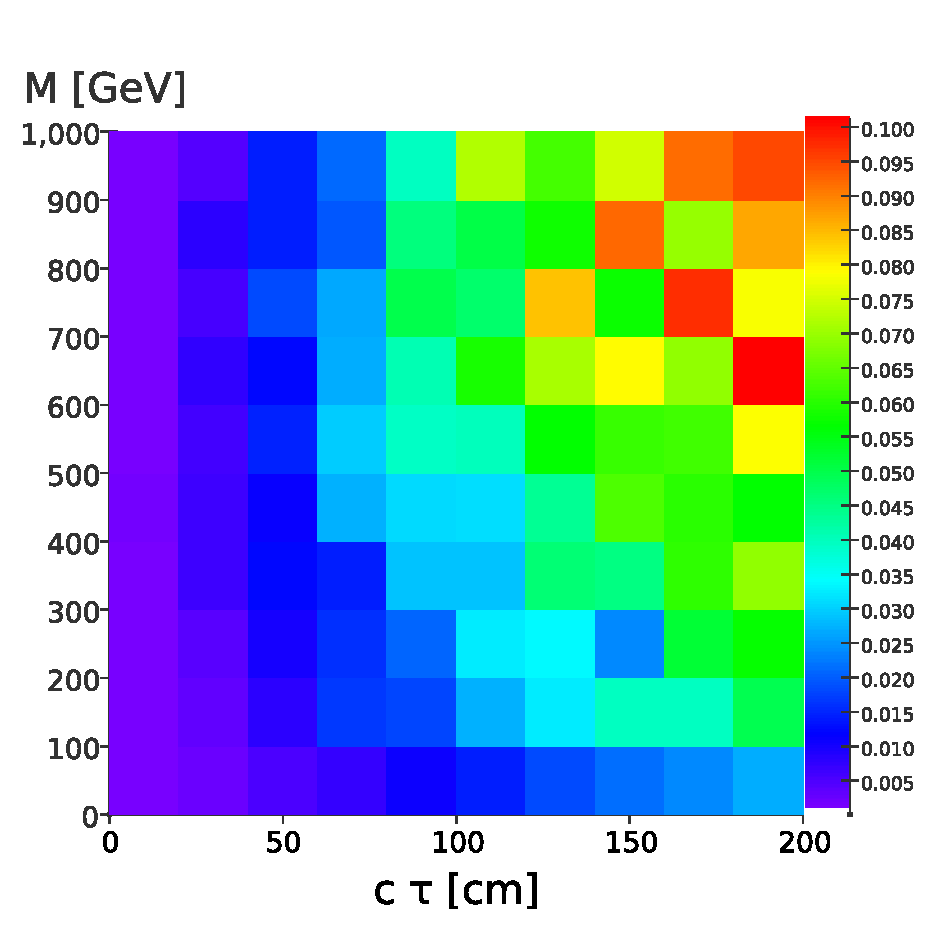
\includegraphics[width=0.4\textwidth]{effic500a.pdf}
   }
   \subfigure[1000 ps] {
   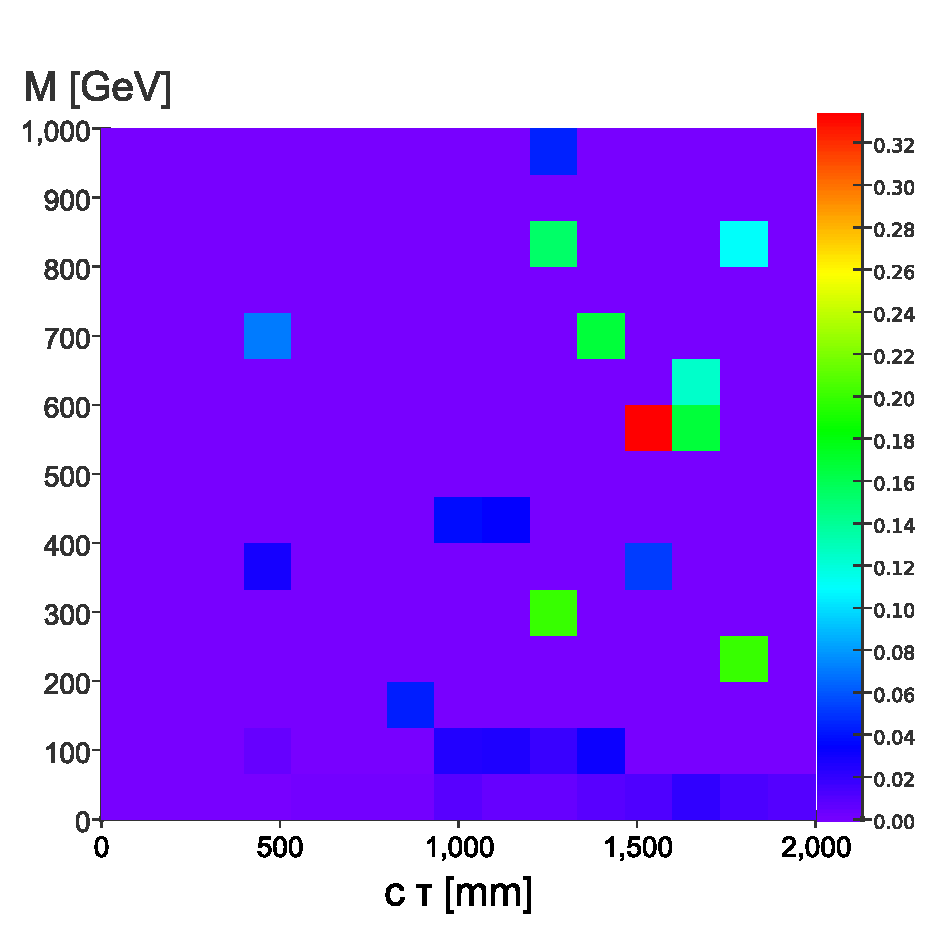
\includegraphics[width=0.4\textwidth]{effic1000a.pdf}\hfill 
   }

\end{center}
\caption{
The acceptance for the reconstruction of emerging jets using the timing layers with different timing resolutions as
a function of the mass of the dark pions and their $c\tau$. The mediator mass was fixed to 10~TeV. The PYTHIA8 simulations are performed 
for the $pp$ collisions at $\sqrt{s}=27$~TeV. 
}
\label{fig:efficiency}
\end{figure}

